\documentclass[border=1cm]{standalone}
\usepackage{tikz}
\begin{document}
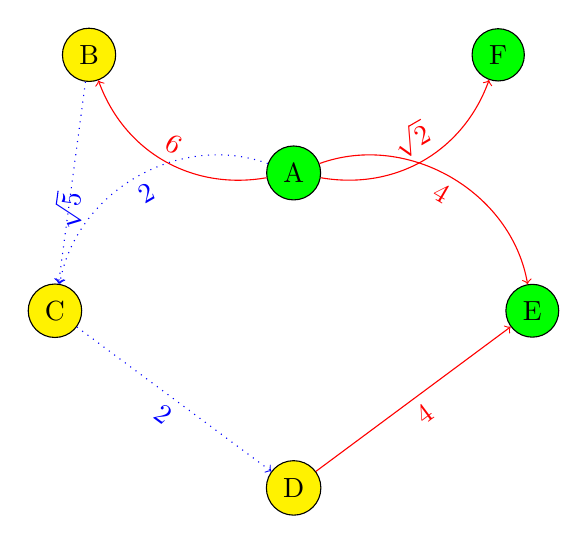
\begin{tikzpicture}
  
  \node[circle, draw, fill=green] (A) at (90:0) {A};
  \node[circle, draw, fill=yellow] (B) at (150:3) {B};
  \node[circle, draw, fill=yellow] (C) at (210:3.5) {C};
  \node[circle, draw, fill=yellow] (D) at (270:4) {D};
  \node[circle, draw, fill=green] (E) at (330:3.5) {E};
  \node[circle, draw, fill=green] (F) at (30:3) {F};

  \draw[->, red] (A) to[bend left=40] node[midway, above, sloped] {6} (B);  
  \draw[->, dotted, blue] (A) to[bend right=50] node[midway, below, sloped] {2} (C);  
  \draw[->, red] (A) to[bend left=50] node[midway, below, sloped] {4} (E);  
  \draw[->, red] (A) to[bend right=40] node[midway, above, sloped] {$\sqrt{2}$} (F);  
  \draw[->, dotted, blue] (B) -- (C) node[midway, left, sloped] {$\sqrt{5}$};  
  \draw[->, dotted, blue] (C) -- (D) node[midway, below, sloped] {2};  
  \draw[->, red] (D) -- (E) node[midway, below, sloped] {4};  
\end{tikzpicture}
\end{document}
